\section{An abstract machine for switches}
\label{s:absmachine}

\begin{figure*}[!t]
  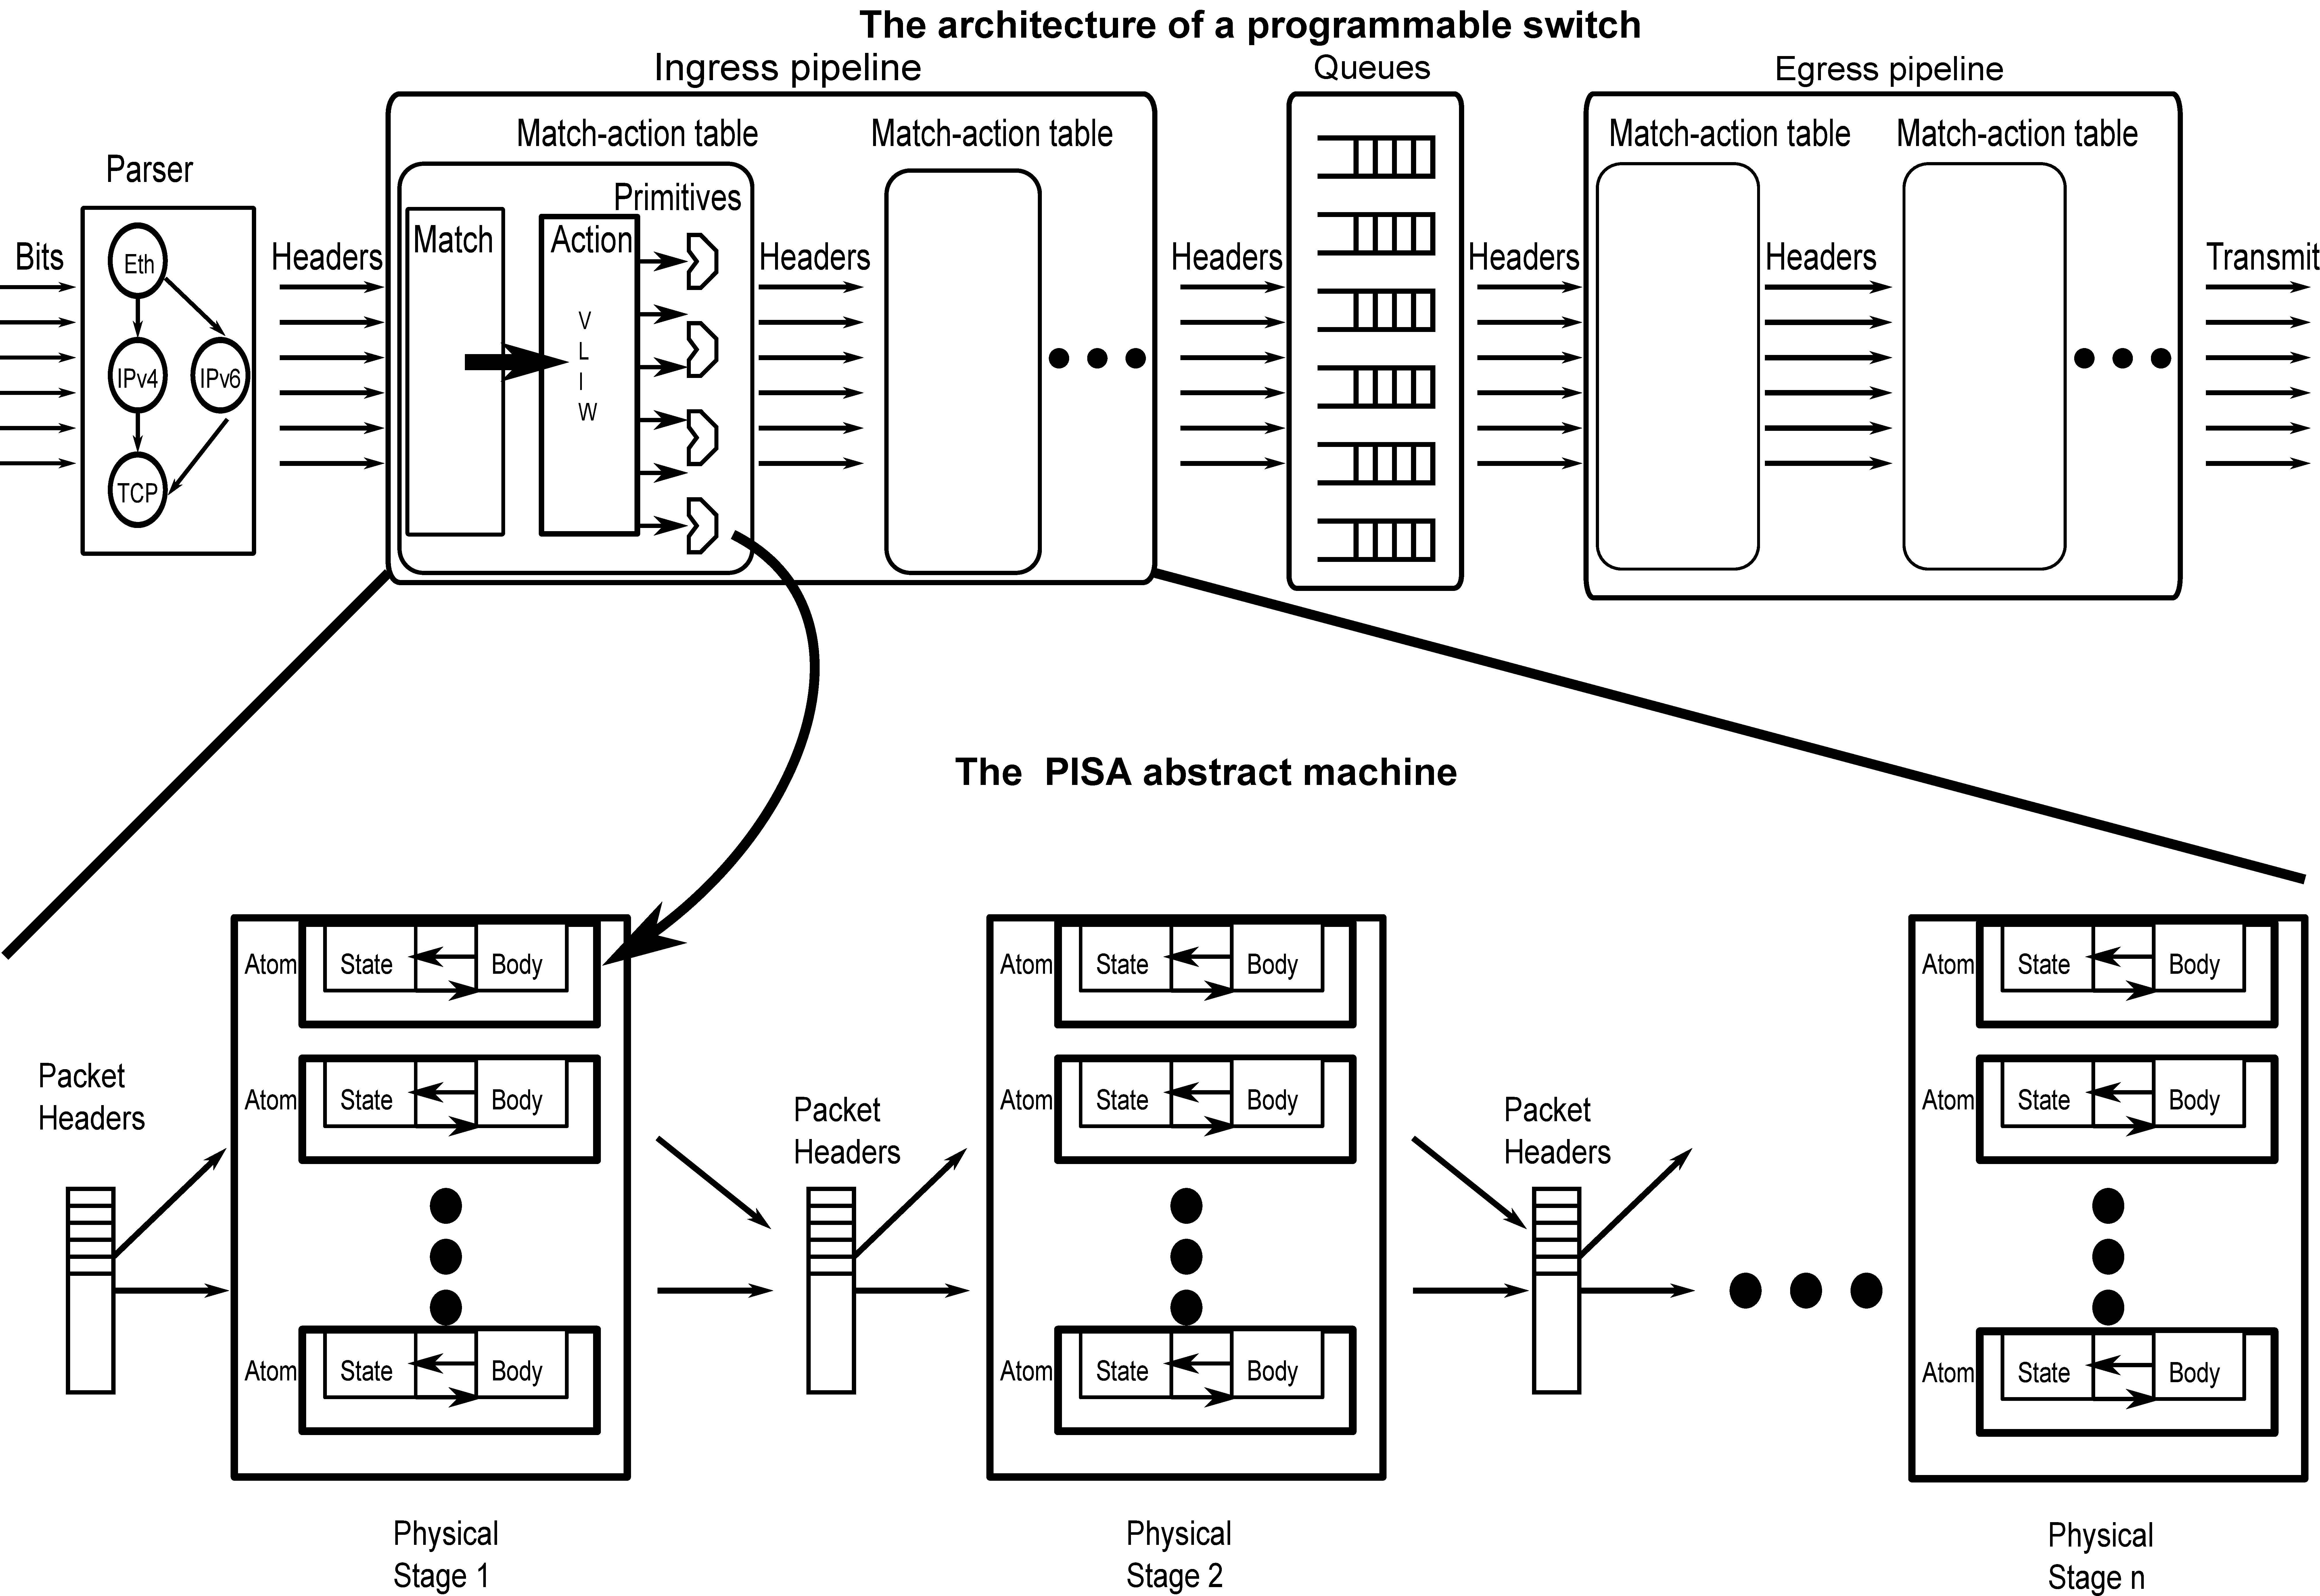
\includegraphics[width=\textwidth]{pisa.pdf}
  \caption{The \absmachine abstract machine and its relationship to
  programmable switch architectures.}
  \label{fig:switch}
\end{figure*}

This section describes \absmachine (Protocol-Independent Switch
Architecture~\cite{nick_p4}), a family of abstract machines for programmable
switches that differ in the computational capabilities they provide.
\absmachine machines serve as compiler targets for \pktlanguage programs.
\absmachine's design is inspired by recent line-rate programmable switch
architectures, such as RMT~\cite{rmt}, Intel's FlexPipe~\cite{flexpipe}, and
Cavium's XPliant Packet Architecture~\cite{xpliant}, which we outline briefly
first.

\subsection{Programmable switch architectures}
Programmable switches follow the switch model shown at the top of
Figure~\ref{fig:switch}.  Packets arriving to the switch are parsed by a
programmable parser that turns packets into header fields. These header fields
are first processed by an ingress pipeline consisting of match-action tables
arranged in stages.  Following the ingress pipeline, the packet is queued. Once
the packet is dequeued by the switch scheduler, it is processed by a similar
egress pipeline before being transmitted from the switch.

\subsection{The \absmachine abstract machine}

\absmachine (the bottom half of Figure~\ref{fig:switch}) models a switch
pipeline such as the ingress or egress pipeline. A pipeline in \absmachine
consists of a number of pipeline stages that execute synchronously on every
time step. An incoming packet is processed by each stage and handed off to the
next, until it exits the pipeline. Each stage has one time step of latency,
where the time step is a physical quantity determined by the hardware. The
inverse of this time step is the line rate supported by the pipeline. For
instance, the RMT architecture has a line rate of 960 Million pkts /
sec~\cite{rmt}.
%TODO: Mention line rate vs. bit rate?

As an abstract machine, \absmachine only models components pertinent to
data-plane algorithms. In particular, it models the computation within a
match-action table in a stage (i.e., the action half of the match-action
table), but not the match semantics (e.g., direct, ternary, or longest prefix).
\absmachine also does not model packet parsing and assumes that packets
arriving to it are already parsed.

\subsection{Atoms: \absmachine's processing units}

In \absmachine, each pipeline stage contains a vector of \textit{atoms}. All
atoms in this vector execute in parallel on every time step.  Informally, an
atom is an atomic unit of packet processing, which the \absmachine machine
supports natively in hardware. We represent an atom as a body of sequential
code. An atom completes execution of this body of code and modifies a packet
before processing the next packet.  An atom may also contain internal state
that persists across packets and influences the atom's behavior from one packet
to the next.  For instance, a switch counter that wraps around at 100 can be
written as the atom below.\footnote{We use {\tt p.x} to represent field {\tt x}
  within a packet {\tt p} and {\tt x} to represent a state variable {\tt x}
that persists across packets.}
  \begin{lstlisting}[style=customc, numbers=none, frame=none]
  if (counter < 99)
    counter++;
  else
    counter = 0;
  \end{lstlisting}
Similarly, a stateless operation that sets a packet field (such as P4's {\tt
modify\_field} primitive~\cite{p4spec}) can be written as the atom below:
\begin{lstlisting}[style=customc, numbers=none, frame=none]
  p.field = value;
\end{lstlisting}

\absmachine generalizes several aspects of existing programmable switch
architectures. The vector of atoms in each stage generalizes RMT's very-large
instruction-word (VLIW)~\cite{rmt} that executes primitive actions on packet
fields in parallel. Internal state within an atom models persistent switch
state such as meters, counters, and P4's register abstraction~\cite{p4spec} in
a unified manner. We assume all state is initialized by the switch control
plane, which we don't explicitly model in \absmachine.

\subsection{Constraining atoms}
\label{s:atomConstraints}

Atoms in \absmachine execute on every time step, reading all packet fields at
the beginning and writing all packet fields at the end of a time step. To
prevent data races, \absmachine forbids two atoms in a stage from writing to
the same packet field.  To provide deterministic performance at line rate,
atoms must be suitably constrained.  We impose two such constraints that
distinguish \absmachine from software routers~\cite{click} and network
processors~\cite{ixp4xx} that sacrifice determinism for programmability.

First, \absmachine machines are \textit{shared-nothing}: each atom maintains a
certain number of state variables that are local to that atom alone. Their
values can be communicated to atoms in subsequent stages only when the values
are copied into packet fields. This restriction reflects the capabilities of
line-rate switches: accessing shared memory from multiple switch stages is
technically challenging because it requires multi-ported RAMs and routing long
wires on the chip.

Second, we constrain the complexity of atoms by defining {\it atom templates}
(\S\ref{ss:code_gen}).  An atom template is a program that always terminates
and specifies how the atom is executed. One example is an ALU with a restricted
set of primitive operations to choose from (Figure~\ref{fig:alu_diag}). Atom
templates allow us to create different \absmachine machines that support
different atoms natively. In practice, we expect such atom templates to be
designed by an ASIC engineer and exposed as part of a \absmachine machine's
instruction set. As programmable switches evolve, the capabilities of atoms
will evolve as well. However, atoms cannot be arbitrarily complex: the line
rate is inversely proportional to an atom's execution
latency~(\S\ref{ss:perfprog}).
